\documentclass[english,11pt]{article}

\pdfoutput=1

\usepackage[T1]{fontenc}
\usepackage[latin9]{inputenc}
\usepackage{verbatim}
\usepackage{float}
\usepackage{amsthm}
\usepackage{amsmath}
\usepackage{amssymb}
\usepackage{graphicx}
%\usepackage{multirow}
\usepackage{color}
\usepackage{url}
\usepackage{caption}
\usepackage{subcaption}
\usepackage{mathtools} 
\usepackage[margin=1.2in]{geometry}

\newcommand{\TODO}[1]{{\color{red}{[#1]}}}

\makeatletter

%%%%%%%%%%%%%%%%%%%%%%%%%%%%%% Textclass specific LaTeX commands.
%\numberwithin{equation}{section}
%\numberwithin{figure}{section}
\theoremstyle{plain}
\newtheorem{thm}{\protect\theoremname}[section]
\theoremstyle{definition}
\newtheorem{defn}[thm]{\protect\definitionname}
\theoremstyle{remark}
\newtheorem{claim}[thm]{\protect\claimname}
\theoremstyle{plain}
\newtheorem{lem}[thm]{\protect\lemmaname}
%
%\newtheorem*{lem*}{Lemma}
%
%\theoremstyle{remark}
%\newtheorem{rem}[thm]{\protect\remarkname}
%\theoremstyle{plain}
%\newtheorem{corollary}[thm]{\protect\corollaryname}
%\theoremstyle{plain}
%\newtheorem{proposition}[thm]{\protect\propositionname}
%%%%%%%%%%%%%%%%%%%%%%%%%%%%%%% User specified LaTeX commands.
%\usepackage{slashbox}

\usepackage{babel}
%\providecommand{\claimname}{Claim}
%\providecommand{\definitionname}{Definition}
%\providecommand{\lemmaname}{Lemma}
%\providecommand{\remarkname}{Remark}
%\providecommand{\theoremname}{Theorem}
%\providecommand{\corollaryname}{Corollary}
%\providecommand{\propositionname}{Proposition}


\newcommand{\reals}{\mathbb{R}}
\newcommand{\RL}{\mathbb{R}^L}
\newcommand{\CL}{\mathbb{C}^L}
\newcommand{\RN}{\mathbb{R}^N}
\newcommand{\RNN}{\mathbb{R}^{N\times N}}
\newcommand{\RLL}{\mathbb{R}^{L\times L}}
%\newcommand{\inner}[1]{\left\langle {#1} \right\rangle}
%\newcommand{\hx}{\hat{x}} 
%\newcommand{\one}{\mathbf{1}} 
\newcommand{\SNR}{{\textsf{SNR}}} 

\begin{document}

\title{Experimental verification}


\author{Tamir Bendory, Nicolas Boumal, William Leeb and Amit Singer}
\maketitle

In this note, we present a preliminary study that aims to show that estimating a particle 
directly from the micrograph, without identifying the location of individual particle images in the micrograph, might be possible. 
In particular, we consider the problem of estimating a set of signals $x_1,\ldots,x_K$ from their multiple occurrences in unknown  locations in a noisy data sequence $y$. Here, $y$ plays the role of the micrograph and the $K$ signals can be thought of as $K$ different viewing directions of the particle, each of which  appears multiple times in the micrograph. 
To be clear, we do not consider here many prominent features of real SPR experiments and do not aim to reconstruct any 3-D structure; instead, we solve a simpler problem that we believe captures key elements of the true SPR problem. 

Figure~\ref{fig:micro_example} shows a simple example of our problem with  one signal ($K=1$). 
Each panel demonstrates an image of size $250\times 250$, containing 4 occurrences of an Einstein image of size $50\times 50$. 
The left panel shows the data without noise. In the middle panel,  i.i.d.\ Gaussian noise with standard deviation $\sigma=0.5$  was added, however,  Einstein is still easily identified. In this scenario it is likely that standard detection algorithms can locate the copies of the signal within the micrograph. In the right panel, we show the same data swamped in  
i.i.d.\ Gaussian noise with standard deviation  $\sigma=3$.
Clearly, identifying the locations of Einstein in this micrograph is much more challenging. In fact, it can be shown that in the low signal--to--noise (\SNR) regime, 
detection  of individual image occurrences is impossible---even if the true image is known---and therefore particle picking is impossible~\cite{aguerrebere2016fundamental}. 
 
\begin{figure}[h!]
	\centering
	\begin{subfigure}[h]{0.33\textwidth}
		\centering
		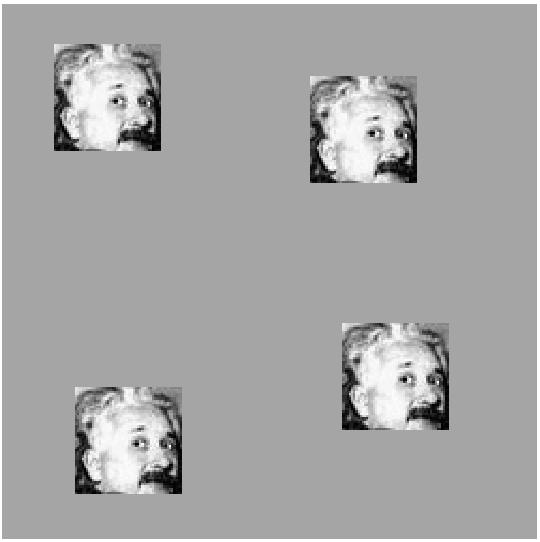
\includegraphics[scale=0.5]{micrograph_Einstein_example_clean}
		\caption{$\sigma = 0$}
	\end{subfigure}%
	\begin{subfigure}[h]{0.33\textwidth}
		\centering
		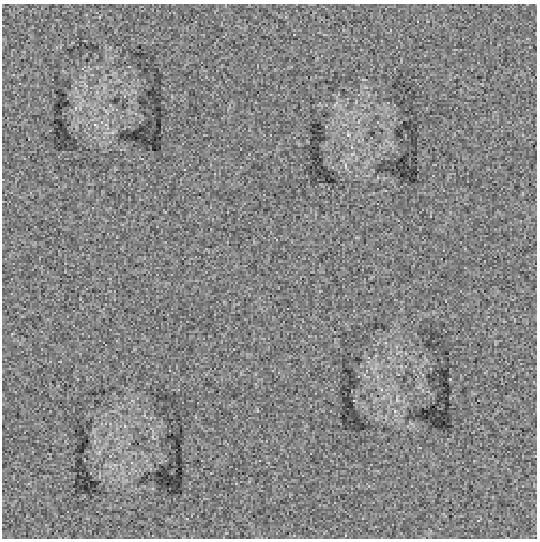
\includegraphics[scale=0.5]{micrograph_Einstein_example_s05}
		\caption{$\sigma = 0.5$}
	\end{subfigure}
	\begin{subfigure}[h]{0.33\textwidth}
		\centering
		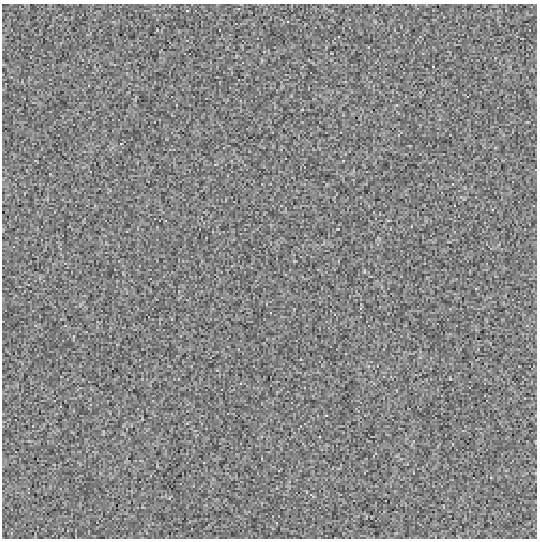
\includegraphics[scale=0.5]{micrograph_Einstein_example_s3}
		\caption{$\sigma = 3$}
	\end{subfigure}
	\caption{\label{fig:micro_example} Example of data sequences (micrographs) of size $250\times 250$ with additive i.i.d.\ Gaussian noise with variance $\sigma^2$. Each micrograph contains four occurrences of a $50 \times 50$ image of Einstein.}	
\end{figure}


\paragraph{Mathematical model}

To be concrete, we formulate the problem for two-dimensional signals. 
Let $x_1,\ldots,x_K\in\RLL$ be the sought signals and let $y\in\RNN$ be the data (i.e., micrograph). 
The forward model can be posed as a mixture of {blind deconvolution} problems between binary signals and the target signals $x_i$:
\begin{equation} \label{eq:model}
y = \sum_{i=1}^K x_i\ast s_i + \varepsilon,\quad \varepsilon\sim\mathcal{N}(0,\sigma^2 I),
\end{equation}
where $\ast$ stands for convolution.
The nonzero values of each  $s_i\in\{0,1\}^{N\times N}$ determine the position of the occurrences of the corresponding $x_i$; see Figure~\ref{fig:micro_example} for an example for $K=1$. We assume a \emph{separation condition} on the binary signals $s=\sum_{i=1}^Ks_i$, that is, the nonzero values of $s$ are separated by at least $L-1$ entries in both axes.

\paragraph{Autocorrelation analysis.}
In order to recover the signals $x_1,\dots,x_K$ from the data, we use autocorrelation analysis.
In a nutshell, the method consists of two stages. First, we estimate a mixture (i.e., linear combination) of the low--order autocorrelation functions of the signals from the data. Then, we estimate the signal itself using non-convex least-squares (LS) or a phase retrieval algorithm. 

\paragraph{Autocorrelation functions.}
We recall that the first-order autocorelation is the mean of the signals. For  
$z\in\RL$ and $k\geq 2$, the autocorrelation of order $k$ is defined for any integer shifts $\ell_1, \ldots, \ell_{k-1}$ by
\begin{align}
a_z^k[\ell_1,\ldots,\ell_{k-1}]  & = \sum_{i=-\infty}^{+\infty} z[i]z[i+\ell_1]\ldots z[i+\ell_{k-1}],
\label{eq:ac_general}
\end{align}
where indexing of $z$ out of the bounds $0, \ldots, L-1$ is zero-padded, as usual.
Explicitly, the first three autocorrelations are
\begin{align} 
a_z^1 & = \sum_{i=0}^{L-1} z[i], \nonumber\\
a_z^2[\ell] & = \sum_{i = \max\{0, -\ell\}}^{L-1 + \min\{0, -\ell\}} z[i]z[i+\ell], \nonumber\\
a_z^3[\ell_1,\ell_2] & = \sum_{i = \max\{0, -\ell_1, -\ell_2\}}^{L-1 + \min\{0, -\ell_1, -\ell_2\}} z[i]z[i+\ell_1]z[i+\ell_2]. \label{eq:ac_special}
\end{align}
The extension to multi-dimensional signals is straight-forward.


\paragraph{Esimtating the mixture of the signals' autocorrelation from the data.}
A mixture of the $K$ signals' autocorrelation functions can be estimated, to any desired accuracy, if individual occurrences are separated by  $L-1$ entries in each direction and each signal appears sufficiently many times in the data. There is no need to detect individual occurrences.

Let $M_i$ denote the number of occurrences of the $i$th signal and  
let us denote
\begin{align}
\gamma_k = \frac{M_k L}{N}.
\end{align}
Then, under the spacing constraint discussed above, one can show that
\begin{align} 
\lim_{N\to\infty} a_y^1 & = \sum_{k=1}^K\gamma_k a_{x_k}^1, \nonumber\\
\lim_{N\to\infty} a_y^2[\ell] & = \sum_{k=1}^K\gamma_k a_{x_k}^2[\ell] +\sigma^2\delta[\ell],  \label{eq:data_ac}\\
\lim_{N\to\infty} a_y^3[\ell_1,\ell_2] & = \sum_{k=1}^K\gamma_k a_{x_k}^3[\ell_1,\ell_2] + \sigma^2\left(\sum_{k=1}^K\gamma_k a_{x_k}^1\right)(\delta[\ell_1,0]+\delta[0,\ell_2]+\delta[\ell_1,\ell_2]). \nonumber
\end{align}
The same  holds for multi-dimensional signals.

\paragraph{Numerical experiments.}
In the first experiment, we estimated Einstein's image from micrographs contaminated with i.i.d.\ Gaussian noise with standard deviation of $\sigma=3$ . An example for such micrograph appears in the right panel of Figure~\ref{fig:micro_example}.

In the experiment, we generated $P$ micrographs, each of size $4000\times 4000$ pixels. 
Within each micrograph, Einstein's images were embedded in random locations, while preserving the separation constraint. On average, each micrograph contains $860$ images. We then computed the first
and second moment of the data and estimated the associated moments of the image using~\eqref{eq:data_ac}. We recall that the second moment is equivalent to the Fourier magnitude of the signal and therefore one can use standard phase retrieval algorithms to recover the signal, up to reflection through the origin. Here, we use an algorithm called relaxed-reflect-reflect (RRR)~\cite{elser2017matrix} that iterates by 
\begin{equation}
x_{\ell+1} = x_\ell  + P_2(2P_1(x_\ell) - x_\ell) - P_1(x_\ell),
\end{equation}
where $P_2(z)$ combines the Fourier phases of $z$ with the Fourier magnitudes estimated from the data, and $P_1$ zeros out the signal out of its support. 

Figure~\ref{fig:Einst_example} shows three example for the reconstructed image using a different number of micrographs. Figure~\ref{fig:error_per_micro}  presents the normalized recovery error as a function of the number of micrographs used in the experiment. The error is computed by 
\begin{equation}
\text{recovery error} = \frac{\|x - \hat{x}\|\|x\|_{\text{F}}}{\|x\|_{\text{F}}},
\label{eq:error}
\end{equation}
where $\hat{x}$ is the estimated image and $\|\cdot\|_{\text{F}}$
denotes the Frobenius norm. We also present the normalized estimation error of the second-moment (power spectrum). The slope in a log-log plot is $-1/2$ as expected. 


\begin{figure}[h!]
	\centering
	\begin{subfigure}[h]{0.25\textwidth}
		\centering
		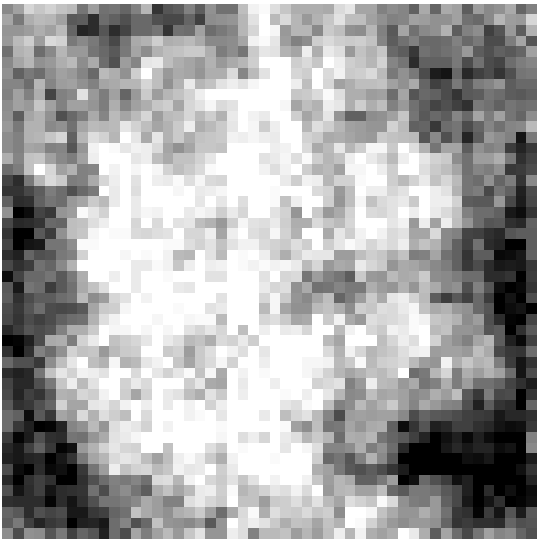
\includegraphics[scale=0.4]{Einstein_100}
		\caption{$P =10^2$}
	\end{subfigure}%
	\begin{subfigure}[h]{0.25\textwidth}
		\centering
		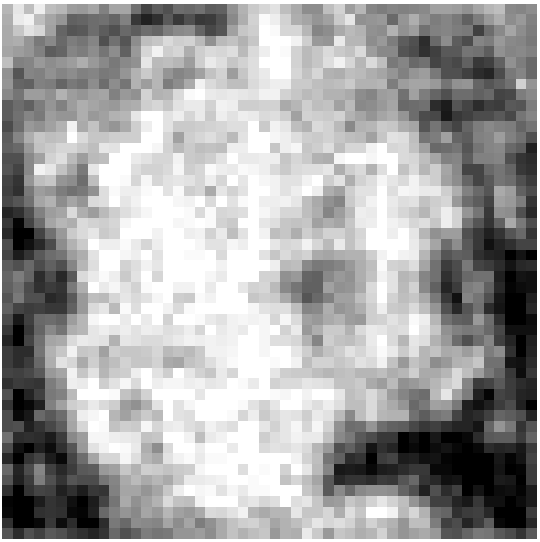
\includegraphics[scale=0.4]{Einstein_1e3}
		\caption{$P =10^3$}
	\end{subfigure}%
	\begin{subfigure}[h]{0.25\textwidth}
		\centering
		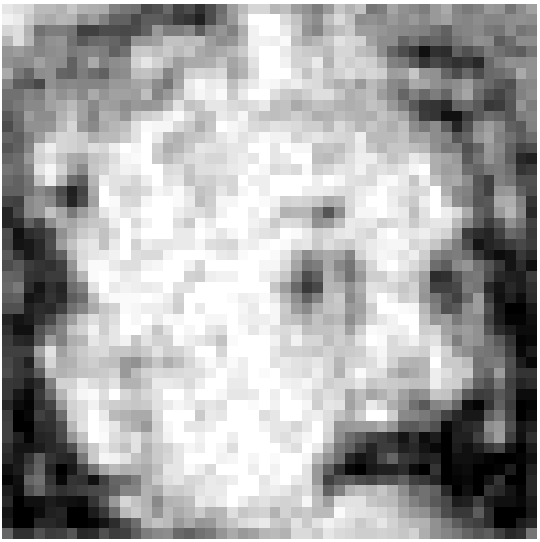
\includegraphics[scale=0.4]{Einstein_1e4}
		\caption{$P = 10^4$}
	\end{subfigure}%
	\caption{\label{fig:Einst_example} Recovery of Einstein image. The algorithm is initialized by the image of Newton. We show estimations of Einstein using $P=10^2,10^3$ and $10^4$ number of micrographs, each contains $860$ image occurrences on average. The normalized recovery error is $0.555$, $0.3988$ and $0.2907$, respectively. The normalized error in recovering the power spectrum was $69.1\times10^{-3} $, $21.7\times10^{-3} $ and $6.8\times10^{-3}$, respectively.}	
\end{figure}


\begin{figure}[h!]
	\centering
	\begin{subfigure}[h]{0.5\textwidth}
		\centering
	 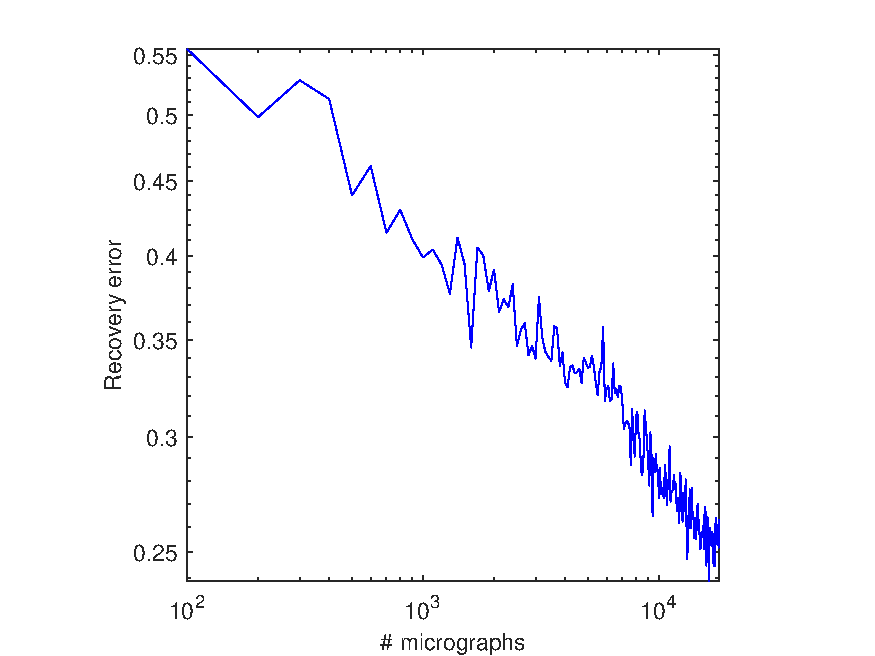
\includegraphics[scale=0.6]{err_rrr_per_micrograph}
    \caption{\label{fig:error_per_micro}}	
	\end{subfigure}%
	\begin{subfigure}[h]{0.5\textwidth}
		\centering
	 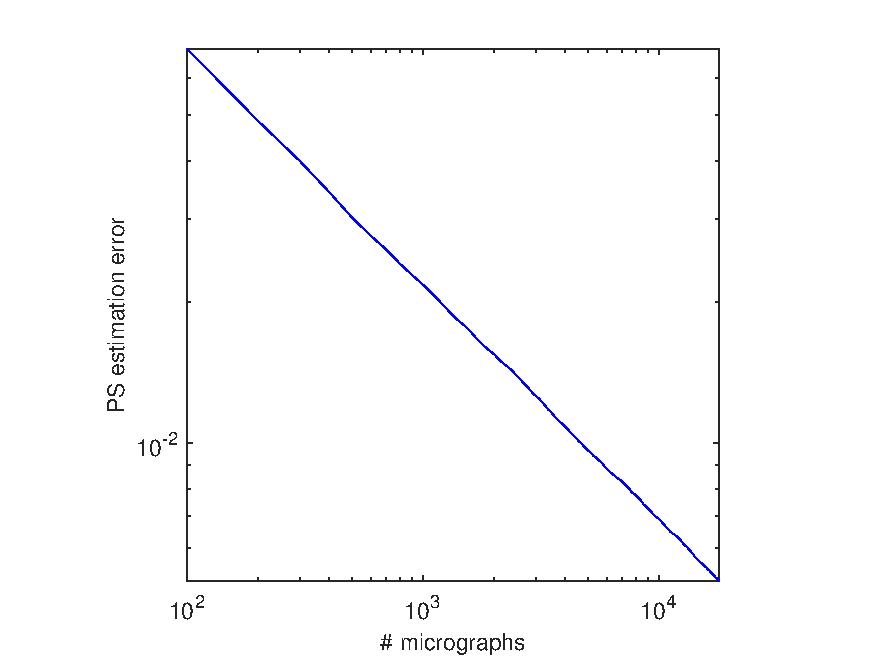
\includegraphics[scale=0.6]{err_PS_per_micrograph}
\caption{}	
	\end{subfigure}%
	\caption{\label{fig:error_per_micro} The left panel shows the recovery error (in log-log scale) of Einstein's image defined~\eqref{eq:error} in as a function of the number of the collected micrographs. The right panel presents the error of estimating the power spectrum of the signal from the data. As expected, in log-log scale, the curve has a $-1/2$ slope.}	
\end{figure}







\bibliographystyle{plain}
\bibliography{ref}

\appendix




\end{document}

